\documentclass[10pt,pdftex,a4paper,twoside,openright]{book}

\usepackage[hmarginratio=3:2, vmargin=1in]{geometry}

%German setting
\usepackage{ngerman}
\usepackage[latin1]{inputenc}
\usepackage[official]{eurosym}
\usepackage[T1]{fontenc}

\usepackage{graphicx}  % Include grafics
\usepackage{grffile}   % support special grafic names
\usepackage{listings}  % Source code

\usepackage{listings}
\usepackage{pdf}
\usepackage{titleref}  % Referenz with name
\usepackage{wrapfig}


\pagestyle{fancy}
% Links nur Kapitel (Gro�keinschreibung statt alles Gro�)
\fancyhead[L]{\nouppercase{\leftmark}}
% Rechts nichts
\fancyhead[R]{}

\usepackage[many]{tcolorbox}
\usepackage{xcolor}
\usepackage{floatflt}
\usepackage{tabularx}
\definecolor{lightyellow}{RGB}{254,254,230}
\newcommand{\ExerciseBox}[1]{
	
	\begin{floatingfigure}[l]{0pt}
		
\includegraphics[scale=0.1]{images/Raspberry-Penguin.png}
	\end{floatingfigure}
			
	\begin{tcolorbox}[colframe=red, colback=lightyellow, boxsep=0mm, arc=3mm, grow to left by=0cm,grow to right by=-0.5cm]
		%
\includegraphics[scale=0.15]{images/Raspberry-Penguin.png}
		
		%\begin{floatingfigure}[l]{0pt}
		%
\includegraphics[scale=0.15]{images/Raspberry-Penguin.png}
		%\end{floatingfigure}
		
		\sffamily{#1}
	\end{tcolorbox}
	\vspace{1cm}
}

\usepackage{blindtext}

\usepackage{pifont,mdframed}

\newenvironment{warning}
{\par
  \begin{mdframed}[linewidth=2pt,linecolor=red]%
		\begin{list}{}{\leftmargin=1cm
				\labelwidth=\leftmargin}\item[\Large]}
		{\end{list}
	\end{mdframed}
	\par}



\setcounter{tocdepth}{2}
\setcounter{secnumdepth}{2} 

\providecommand{\versionnumber}{19.10}


\title{Raspberry Pi Jam - Raspjamming}
\author{\textbf{Autoren und Mitwirkende:}\\
	Martin Strohmayer\\
	Christoph W�rg�tter\\
	Christof Hirndler\\
	Manfred Wallner\\
}
\date{Version \versionnumber \\\today \\PDF Edition}

\begin{document}

\maketitle

\tableofcontents

\chapter{Installation Raspberry Pi}

\section{Raspbian}


Raspbian ist das offizielle Betriebssystem f�r den Raspberry~Pi. F�r die Verwendung bei einem Raspberry Pi Jam wurde ein eigenen Image vom Grazer Computer Club (GC2) mit dem Namen Raspjamming erstellt und zur Verf�gung gestellt. Ausgehend vom 
Raspbian Lite Image wurde noch verschiedene Entwickerlerprogramm und Werkzeuge installiert. Zus�tzlich wurde das System so eingerichtet, dass die Raspberry Pi Zero direkt �ber den USB-OTG Anschluss mit dem Host PC verbunden werden kann. Der SSH-Dienst und WLAN wurde aktiviert. Alle L�ndereinstellung wurden  von UK auf �sterreich/German ge�ndert. Ein Web-Server stellt Programme und Hilfe zur Verf�gung, auch ohne Internet..\\  
F�r die Installation ben�tigt man ein beliebiges Linux System mit einem MicroSD-Kartenleseger�t.  Es wird mindestens eine 4~GB gro�e MicroSD-Karte ben�tigt. Die aktuelle Raspjamming Version kann als Image-Datei von der Seite \url{https://github.com/GrazerComputerClub/Raspjamming-Image} heruntergeladen werden. 

\begin{console}
	wget --trust-server-names http://www.strohmayers.com/image/2019-02-07-Raspjamming-full.zip
	unzip 2019-02-07-Raspjamming-full.zip
	rm 2019-02-07-Raspjamming-full.zip
\end{console}


\subsection{Etcher}

Das grafische Programm Etcher (\url{https://etcher.io}) kann zum �bertragen der Image-Datei verwendet werden. Es ist vor Allem f�r Anf�nger zu empfehlen, da beim Konsolenprogramm dd das Risiko besteht, dass Daten einer falschen Partition bzw. eines Laufwerks zerst�rt werden. Das Programm muss allerdings manuell installiert werden.     

\begin{console}
	wget https://github.com/resin-io/etcher/releases/download/v1.3.1/etcher-1.3.1-linux-x86_64.zip 
	unzip etcher-1.3.1-linux-x86_64.zip
	chmod +x etcher-1.3.1-x86_64.AppImage
	sudo mv etcher-1.3.1-x86_64.AppImage /usr/local/bin/etcher
	etcher &
\end{console}


Nach dem Starten wird danach gefragt ob eine Verkn�pfung zum Programm erstellt werden soll. Dies sollte man mit "`Yes"' beantworten. Danach kann man mit der Schaltfl�che "`Image"' die Image-Datei ausw�hlen. Ist nur ein m�gliches Ziel vorhanden, wird es bereits vorausgew�hlt, z.~B. die SD-Karte im Karten-Slot (/dev/memcblk0) oder im USB-Adapter (/dev/sdb). Sind mehrere m�gliche Ziele vorhanden, wird die "`Select Drive"' Schaltfl�che freigeschaltet. Dann kann ein Laufwerk manuell ausgew�hlt werden.

\begin{figure}[ht]
	\centering
	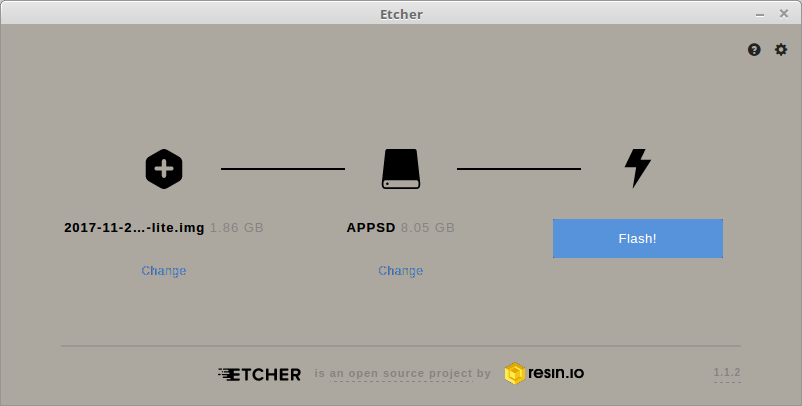
\includegraphics[scale=0.3]{images/Etcher_1.png}
	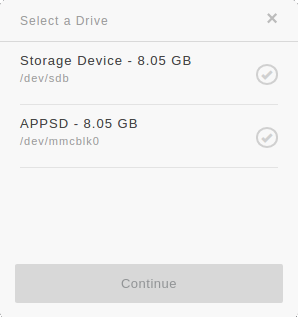
\includegraphics[scale=0.3]{images/Etcher_2.png}
	\label{Etcher}
\end{figure}


Wenn man noch etwas �ndern will, kann die entsprechende "`Change"' Schaltfl�che ausgew�hlt werden. Zum Schluss wird der Schreibvorgang mit der "`Flash!"' Schaltfl�che gestartet. M�glicherweise wird vom Programm allerdings noch das System-Passwort abgefragt.\\ 
Das Laufwerk bzw. die Partitionen werden nun aus dem System ausgeh�ngt und der Schreibvorgang gestartet. Der Fortschritt, die durchschnittliche �bertragungsrate und die Restlaufzeit werden w�hrend des Vorgangs angezeigt.\\ 


\subsection{dd Kommandozeilenprogramm}

Die erhaltene Image-Datei kann mit dem Kommandozeilenprogramm dd auf eine MicroSD-Karte �bertragen werden.\\
\textbf{Es ist unbedingt vor dem Ausf�hren des Befehls zu pr�fen, ob das angegebene Laufwerk bzw. Device auch der vorgesehenen MicroSD-Karte entspricht!}\\ 
Bei USB-Kartenlesern bzw. USB-Adaptern ist die Ermittlung des Devices leicht �ber die Systemmeldungen m�glich. 

\begin{console}
	dmesg | tail -n 10
\end{console}

\begin{screensmall}
	scsi 3:0:0:0: Direct-Access     MXT-USB  Storage Device   1308 PQ: 0 ANSI: 0 CCS
	sd 3:0:0:0: Attached scsi generic sg1 type 0
	sd 3:0:0:0: [sdb] 15730688 512-byte logical blocks: (8.05 GB/7.50 GiB)
	sd 3:0:0:0: [sdb] Write Protect is off
	sd 3:0:0:0: [sdb] Mode Sense: 03 00 00 00
	sd 3:0:0:0: [sdb] No Caching mode page found
	sd 3:0:0:0: [sdb] Assuming drive cache: write through
	sdb: sdb1 sdb2
	sd 3:0:0:0: [sdb] Attached SCSI removable disk
	EXT4-fs (sdb2): mounted filesystem with ordered data mode. Opts: (null)
\end{screensmall}

Die MicroSD-Karte wurde im Beispiel als Device "`sdb"' �ber einen USB-Adapter eingebunden. Nun kann man die Image-Datei mit dem Programm dd auf die MicroSD-Karte �bertragen. Mit dem Parameter "`of"' muss der komplette Device-Name, in diesem Fall "`/dev/sdb"', angegeben werden. Bei Parameter "`if"' wird die entpackte Image-Datei angeben. Die Bl�ckgr��e bzw. der Cache wird mit Parameter "`bs"' gesetzt. Eine gr��ere Blockgr��e erh�ht die Schreibgeschwindigkeit. Sie wird im Beispiel mit 4~MB angegeben.\\
Zu Beachten ist, dass der USB-Massenspeicher m�glicherweise bereits automatisch gemountet wurde. Dann sollte man die Partitionen mit dem Befehl "`umount"' zuerst auswerfen. 


\begin{console}
	umount /dev/sdb1 /dev/sdb2
	dd if=2019-02-07-Raspjamming-full.img of=/dev/sdc bs=4M
\end{console}

\begin{screensmall}
	2623+0 Datens�tze ein
	2623+0 Datens�tze aus
	2387266048 Bytes (2,4 GB) kopiert, 247,6147 s, 10,4 MB/s
\end{screensmall}


\section{USB Gadget / OTG Modus Raspberry Pi Zero}


F�r den USB Gadget Modus der Raspberry Pi Zero wird bereits eine vorkonfigurierte MicroSD-Karte bzw. ein MicroSD-Karten-Image zur Verf�gung gestellt. Darauf sind bereits alle Voreinstellungen durchgef�hrt worden.\\
\textbf{Sollte die Einrichtung manuell erfolgen oder wird Microsoft Windows als Host verwendet, so muss man sich das PDF-Dokument 'Raspberry Pi Jam - Raspjamming Admin' besorgen.} 

\subsection{Host (DHCP-Client)}
%\clearpage
\subsubsection{Kubuntu 16.04}

Am Host-PC muss bei den IPv4-Einstellungen die Methode "`Automatisch"' eingestellt sein. Wenn es sich um eine neue Verbindung handelt, ist dies bereits voreingestellt, eine Parametrierung kann dann entfallen. Ansonsten muss zur Konfiguration unter Linux (Kubuntu 16.04) zuerst der Dialog "`Netzwerkverbindungen"' ge�ffnet werden.\\ 
Dazu klickt man mit der rechten Maustaste auf das Netzwerksymbol in Infobereich rechts unten. Dann kann die Option "`Netzwerkverbindungen einrichten..."' ausgew�hlt werden.

\begin{figure}[ht]
  \centering
  
\includegraphics[scale=1.00]{images/OTG_NetzwerkverbindungenIcon.png}	
  
\includegraphics[scale=0.42]{images/OTG_NetzwerkverbindungenOpen.png}	
  %	\caption{}
  \label{OTG_LINUX_NetzwerkverbindungenApp}
\end{figure}


Nun k�nnte die neue "`Kabelnetzwerkverbindung"' umbenannt werden, z.~B. in Raspberry Pi Zero. Erkennen kann man das Netzwerk an der Mac-Adresse, die man bei "`g\_ether.host\_addr"' angegeben hat (z.~B. 00:01:02:03:04:05).  


\begin{figure}[ht]
  \centering
  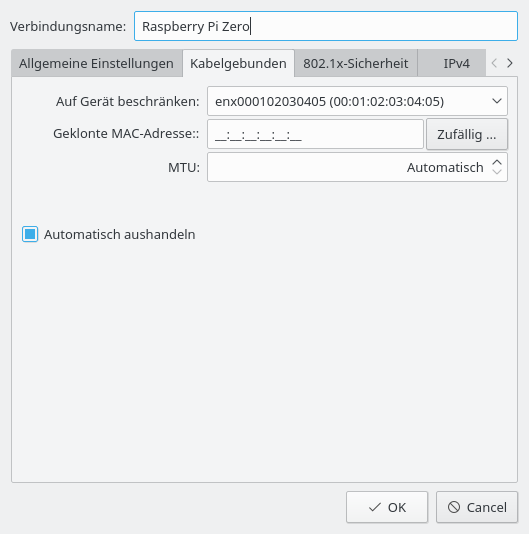
\includegraphics[scale=0.42]{images/OTG_Pi_Verbindungsname.png}
	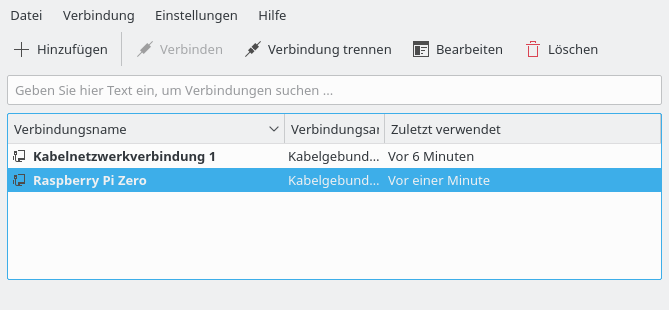
\includegraphics[scale=0.42]{images/OTG_Netzwerkverbindungen.png}
%	\caption{}
  \label{OTG_LINUX_Netzwerkverbindungen}
\end{figure}


Nun kann bei den IPv4-Einstellungen die Methode "`Automatisch"' eingestellt werden.

%\begin{figure}[ht]
%  \centering
%  \includegraphics[scale=0.42]{images/OTG_NetzwerkverbindungenAutomatisch.png}
%	\caption{}
%  \label{OTG_LINUX_Netzwerkverbindungen}
%\end{figure}

%\clearpage
%\input{OTG_Mint}

%\subsection{Internet Zugriff} 
~\\
Nach der Einrichtung des Netzwerk kann der Raspberry Pi Zero mit dem Namen "`raspberrypi.local"' erreicht werden. Um den Raspbery Pi Zero mit dem Internet verbinden zu k�nnen m�ssen einige Einstellungen am Host %und Client
 gemacht werden. Man muss den Name des Netzwerkger�ts am Host-PC kennen, das mit dem Internet verbunden ist. Dies ermittelt man �ber die Netzwerkeinstellungen oder �ber die Konsole mit nmcli. Im Beispielfall ist der Name "`enp0s25"' das richtige Ger�t.

\begin{console} 
	nmcli d
\end{console} 

\begin{screensmall} 
	GER�T            TYP       STATUS           VERBINDUNG        
	enx000102030405  ethernet  verbunden        Raspberry Pi Zero 
	enp0s25          ethernet  verbunden        Netzwerkverbindung 1                
	lo               loopback  nicht verwaltet  --  
\end{screensmall}

Damit der Internetzugang f�r den Raspberry Pi Zero freigegeben wird, m�ssen am Host-PC folgende Befehle in einem Terminal eingeben werden. "`enp0s25"' muss durch den Namen des Netzwerkger�ts ersetzt werden, das mit dem Internet verbunden ist.

\begin{console} 
	sudo sysctl -w net.ipv4.ip_forward=1
	sudo iptables -t nat -A POSTROUTING -o enp0s25 -j MASQUERADE
\end{console}



Alternativ k�nnen die Einstellungen auch automatisch �ber eine Shell-Script durchgef�hrt werden (siehe Kapitel \ref{sec:shellscript} \titleref{sec:shellscript}).


\section{Verbindung}

\subsection{SSH}

Nach der Einrichtung kann per SSH-Client eine Verbindungen zum Raspberry Pi hergestellt werden. Dazu muss in einem Terminal folgender Befehl eingegeben werden:

\begin{console} 
	ssh -X pi@raspberrypi.local
\end{console}

Um grafische Programme am Host anzeigen zu k�nnen, muss der Parameter \texttt{-X} angegeben werden. "`\textbf{pi}"' ist der Standardbenutzer am System. Dann wird eine X-Server Verbindung via SSH hergestellt. Verbindet man sich zum ersten Mal mit dem Raspberry Pi, so wird noch eine Sicherheitswarnung ausgegeben. Der kryptographische Schl�ssel f�r die Verbindung ist dem lokalen System noch nicht bekannt.%  und muss best�tigt werden.
\begin{screensmall}
The authenticity of host 'raspberrypi.local (192.168.137.10)' can't be established.
ECDSA key fingerprint is SHA256:Dcf3HYgE2GHnNnZ8Xhv8iJ9yA+zvfXBC9COm2eL9i0w.
Are you sure you want to continue connecting (yes/no)? 
Warning: Permanently added 'raspberrypi.local,192.168.137.10' (ECDSA) to the list of known hosts.
\end{screensmall}

Die Frage muss mit \texttt{yes} best�tigt werden. Anschlie�end muss das Default-Passwort von Raspbian "`\textbf{raspberry}"' eingegeben werden. Nun sollte man den Raspberry Pi Prompt \texttt{pi@rasbperrypi:\textasciitilde  \$} sehen. 

Wechselt man zu einem anderen Raspberry Pi mit den gleichen Namen oder installiert das System nochmals, so kann es passieren, dass eine Fehlermeldung ausgegeben wird, weil sich der kryptographische Schl�ssel ge�ndert hat.

\begin{screensmall} 
@@@@@@@@@@@@@@@@@@@@@@@@@@@@@@@@@@@@@@@@@@@@@@@@@@@@@@@@@@@
@    WARNING: REMOTE HOST IDENTIFICATION HAS CHANGED!     @
@@@@@@@@@@@@@@@@@@@@@@@@@@@@@@@@@@@@@@@@@@@@@@@@@@@@@@@@@@@
\end{screensmall} 

%The ECDSA host key for raspberrypi.local has changed,
%and the key for the corresponding IP address 169.254.229.192
%is unknown. This could either mean that
%DNS SPOOFING is happening or the IP address for the host
%and its host key have changed at the same time.
%@@@@@@@@@@@@@@@@@@@@@@@@@@@@@@@@@@@@@@@@@@@@@@@@@@@@@@@@@@@
%@    WARNING: REMOTE HOST IDENTIFICATION HAS CHANGED!     @
%@@@@@@@@@@@@@@@@@@@@@@@@@@@@@@@@@@@@@@@@@@@@@@@@@@@@@@@@@@@
%IT IS POSSIBLE THAT SOMEONE IS DOING SOMETHING NASTY!
%Someone could be eavesdropping on you right now (man-in-the-middle attack)!
%It is also possible that a host key has just been changed.
%The fingerprint for the ECDSA key sent by the remote host is
%SHA256:Dcf2HYyE2GHnNpZ8Xhv8iJ9yj+zvfXBC9COm2eL9i0w.
%Please contact your system administrator.
%Add correct host key in /home/evil/.ssh/known_hosts to get rid of this message.
%Offending ECDSA key in /home/evil/.ssh/known_hosts:9
%remove with:
%ssh-keygen -f "/home/evil/.ssh/known_hosts" -R raspberrypi.local
%ECDSA host key for raspberrypi.local has changed and you have requested strict checking.

In diesem Fall muss man die Verbindung aus den bekannten Hosts l�schen. Hierf�r muss folgendes Kommando ausgef�hrt werden:

\begin{console} 
	ssh-keygen -R raspberrypi.local
\end{console}

Optional kann auch der Parameter \texttt{-o UserKnownHostsFile=/dev/null} beim ssh-Befehl hinzugef�gt werden. Dann erfolgt keine �berpr�fung der Verbindung. 


\subsection{SSH �ber Shell-Script} \label{sec:shellscript}

Das Einfachste ist die Verbindung zu Raspberry Pi �ber das vorbereitete PiConnect.sh Shell-Script herzustellen. Es setzt automatisch die Internetweiterleitung und startet die SSH-Verbindung. Es kann vom vorbereitetet Raspbian-Image oder von Github geladen werden.

\begin{console} 
	scp pi@raspberrypi.local:/home/pi/scripts/PiConnect.sh .
\end{console}
oder
\begin{console} 
	wget --trust-server-names https://goo.gl/uwguQo
	sh PiConnect.sh
\end{console}   




\section{Einstellungen}


Als erstes kann das Raspberry Pi Software Configuration Tool (raspi-config)  gestartet werden. Dazu verwendet man den Aufruf "`sudo raspi-config"'.\\
Der Men�punkt "`Change User Password"' �ndert das Passwort f�r den Benutzer "`pi"'.\\
Danach sollte man die Regionseinstellungen mit dem Men�punkt "`Localisation Options"' einstellen. Im folgenden Untermen� kann man mit "`Change Locale"' die Sprache und Zeichensatz des Systems setzen. Hier w�hlt man z.~B. "`de\_AT.UTF-8 UTF8"' f�r �sterreich oder "`de\_DE.UTF-8 UTF8"' f�r Deutschland. "`en\_GB.UTF-8 UTF8"' und  "`C.UTF-8"' sind bereits ausgew�hlt und k�nnen zus�tzlich aktiv sein. Im n�chsten Fenster kann man dann die Sprache "`de\_AT.UTF-8 UTF8"' bzw. "`de\_DE.UTF-8 UTF8"' als Standardeinstellung �bernehmen.\\ 
Nun kann man mit "`Change Timezone"' die aktuelle Zeitzone ausw�hlen. F�r das geografische Gebiet kann man "`Europe"' ausw�hlen. Danach kann man als Zeitzone die Stadt "`Vienna"' oder "`Berlin"' ausw�hlen.\\
Bei der dritten Einstellung "`Change Keyboard Layout"' kann man das Tastatur-Layout aktualisieren.
%ausw�hlen:\\
%Keyboard model: Generic 105-key (Intl) PC \textit{(Tastatur mit Windows Taste)}\\
%Keyboard layout: Other\\
%Country of origin for the keyboard: German\\
%Keyboard layout: German - German (eliminate dead keys)\\
%Key to function as AltGr: The default for the keyboard layout\\
%Compose key: No compose key\\
%Use Control+Alt+Backspace to terminate the X server?: <Yes>\\


\section{Aktualisierungen und Programme}


Beim Raspjamming Image wurden die Programmiersprachen und Entwicklungswerkzeuge Python, Python 3, C/C++, C\# (Mono) und Blockly-gPIo installiert. Zus�tzlich sind auch Raspberry Pi Bibliotheken f�r die Entwicklungswerkzeuge vorinstalliert.\\
F�r das Arbeiten mit Microkontrollern (AVR und ESP) wurden Compiler, Tools und  serielle Terminalprogramme installiert.\\
Zur Versionsverwaltung wurde git installiert. Als Editor bzw. als einfache IDE ist Geany verf�gbar.\\

Die Abk�rzung \textit{IDE} bezeichnet eine integrierte Entwicklungsumgebung (Integrated Development Environment). Sie stellt umfassende Funktionen und Programme zur Entwicklung von Programmen bereit. Die Hauptkomponenten sind Editor, Compiler und Debugger.\\  
Eine Versionsverwaltung ist ein System, das zur Verwaltung, Archivierung und Erfassung von �nderungen an Source-Dateien verwendet wird. GitHub ist ein webbasierter Online-Dienst zur Versionsverwaltung, der viele Software-Entwicklungsprojekte bereitstellt.\\
%\textit{CodeLite} ist eine freie plattform�bergreifende IDE, die auf die Programmiersprachen C, C++, PHP und JavaScript (Node.js) spezialisiert ist. \textit{Code::Blocks} ist eine freie plattform�bergreifende IDE f�r die Programmiersprachen C, C++ und Fortran.\\
\textit{Geany} ist ein Texteditor mit grundlegenden Funktionen. Es wurde entwickelt, um eine kleine und schnelle IDE bereitzustellen. Nachteil gegen�ber einer IDE wie \textit{CodeLite} oder \textit{Code::Blocks} ist vor allem das Fehlen eines Debuggers und Probleme bei multiplen Projektdateien. Der Benutzer muss sich darum k�mmern, dass die Kompileranweisung alle Sourcecode Komponenten einschlie�t. Kompilierfehler werden im Source nicht hervorgehoben, sondern nur in einem Fester ausgegeben. F�r die einfachen Beispiele in dieser Anleitung ist es aber gut geeignet. Das Programm unterst�tzt alle wichtigen Entwicklungsumgebungen wie C, C++, C\# und Python.\\
\textit{WiringPi} und \textit{pigpio} sind zwei C-Bibliotheken, die das Arbeiten mit den GPIOs der Raspberry Pi erm�glichen. Sie sind nicht kompatibel, man muss sich also f�r eine entscheiden. In der Anleitung wird ausschlie�lich die \textit{WiringPi} Bibliothek benutzt. \textit{git} ist ein Versionsverwaltungsystem das Zugriff auf Source-Dateien von Projekte erm�glicht. Diese werden zumeist auf Online-Dienst GitHub zur Verf�gung gestellt. Das Paket \textit{build-essential} enth�lt GNU C und C++ Compiler sowie die GNU-C-Bibliothek um C/C++-Projekte kompilieren bzw. erstellen zu k�nnen.\\ 
\textit{minicom} und \textit{screen} sind Programme, um auf der seriellen Schnittstelle (UART) der Raspberry Pi kommunizieren zu k�nnen.\\
\textit{python-dev} bzw. \textit{python3-dev} enth�lt Bibliothek und Entwicklungswerkzeuge zum Erstellen von Python-Scripte, sowie den Python-Interpreter selbst. In der Anleitung wird ausschlie�lich die aktuelle Version 3 von Python verwendet. \textit{rpi.gpio} ist eine Python Bibliothek die Basisfunktionalit�ten der GPIOs unterst�tzt. \textit{gpiozero} ist eine aktuelle Python Bibliothek die viele Funktionen der GPIOs zur Verf�gung stellt und von der Raspberry Pi Foundation empfohlen wird. Bei den Beispielen wird ausschlie�lich diese Library verwendet.\\
\textit{mono-complete} enth�lt Compiler, Librarys und die Runtimeumgebung um CIL (Common Intermediate Language) Bytecode, auch als Assemblies bekannt, erzeugen und ausf�hren zu k�nnen. Es wird f�r die Erstellung von C\# Programmen ben�tigt.

\subsection{Geany - Entwicklungsumgebung}

Nach dem Herstellen der Verbindung zur Raspberry Pi �ber SSH, kann die grafische Entwicklungsumgebung Geany gestartet werden.

\begin{console}
	cd ~
	geany &
\end{console}

Soll Geany in Englisch ausgef�hrt werden obwohl das System auf Deutsch gestellt wurde, so muss man vor dem Start die Variable "`LANG"' auf "`C"' setzen.

\begin{console}
	LANG=C geany &
\end{console}

Nun kann eine Source-Datei geladen oder erstellt werden. Dann kann das Konfigurationsfenster ge�ffnet werden, indem man im Men� unter \texttt{Erstellen} $\rightarrow$ \texttt{Kommandos zum Erstellen konfigurieren} ausw�hlt.\\
Die Parameter f�r \texttt{Kompilieren} und \texttt{Erstellen} werden bereits anhand der Source-Datei (Extention) vorbelegt. Zumeist m�ssen aber noch Anpassungen vorgenommen werden, um Bibliotheken oder ge�nderte Kompiler verwenden zu k�nnen. Werden zwei Source-Dateien im Projekt ben�tigt, so m�ssen auch beide in der Anweisung vorkommen ("'g++ -o Zieldatei Quelldatei1.cpp Quelldatei2.cpp"'). Es k�nnen Platzhalter mit verschiedenen Funktionen eingef�gt werden. \texttt{\%f} wird durch den Dateinamen der im Editor ausgew�hlten Datei ersetzt. \texttt{\%e} wird durch den Dateinamen ohne Extention der im Editor ausgew�hlten Datei ersetzt.\\   
%f - replaced by the filename of the file selected in the editor when the menu item is selected.
%e - replaced by the same filename but without the last extension.
Was genau bei den Feldern einzutragen ist, wird in den folgenden Beispielprogrammen der einzelnen Programmiersprachen angegeben.\\    

Danach kann das Programm mit der Taste \texttt{Erstellen} erzeugt werden und mit der Taste \texttt{Ausf�hren} in einem Terminal gestartet werden.\\
Die Tastenk�rzel f�r alle Funktionen k�nnen �ber das Men� \texttt{Bearbeiten} $\rightarrow$ \texttt{Einstellungen} $\rightarrow$ \texttt{Tastenk�rzel} vorgegeben werden. Dazu w�hlt man die gew�nschte Aktion aus und dr�ckt die Taste "`�ndern"'. Danach kann man die Taste bzw. Tastenkombination dr�cken, die dann umgehend im Dialog angezeigt wird. Wenn nun die OK-Taste gedr�ckt wird, wird die �nderung �bernommen und das Tastenk�rzel f�hrt in Zukunft die Aktion aus. 
Im Beispiel wurde der Aktion "`Erstellen"' dem Tastenk�rzel bzw. der Taste \framebox{F7} zugewiesen.\\ 
Eine Beschreibung zur Erstellung und Parametrierung eines Projekts kann dem Kapitel \ref{sec:Projekt_LED} \titleref{sec:Projekt_LED} bzw. \ref{sec:Projekt_Ampel} \titleref{sec:Projekt_Ampel} 
entnommen werden.

\begin{figure}[ht]
  \centering
  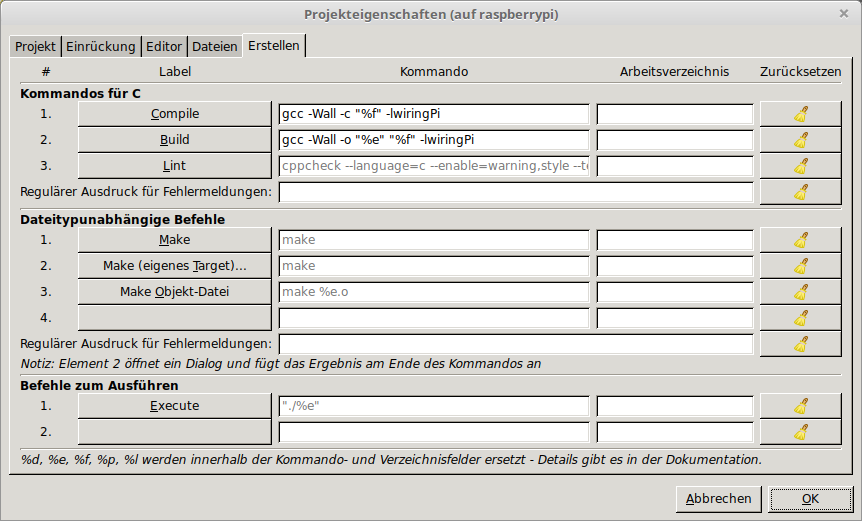
\includegraphics[scale=0.48]{images/Geany_Create.png}
  \caption{Kommandos zum Erstellen konfigurieren f�r C Projekt}
  \label{Geany-create}
\end{figure}

\begin{figure}[ht]
  \centering
  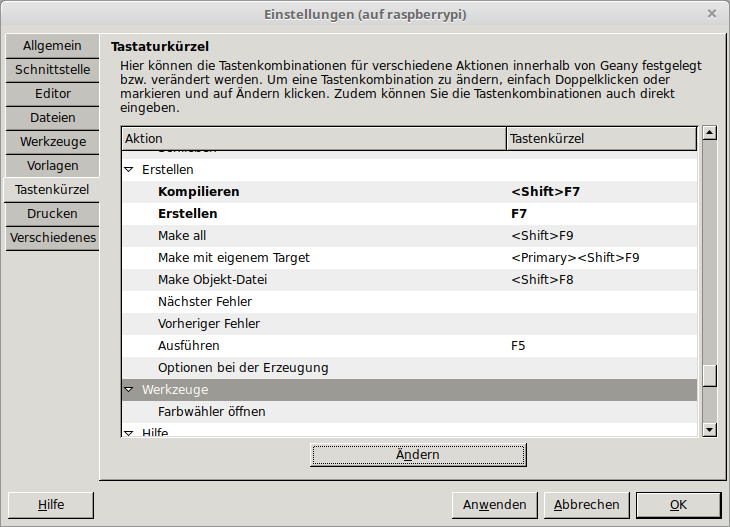
\includegraphics[scale=0.48]{images/Geany_Settings.png}
  \caption{Tastaturk�rzel}
  \label{Geany-settings}
\end{figure} 

\begin{figure}[ht]
  \centering
  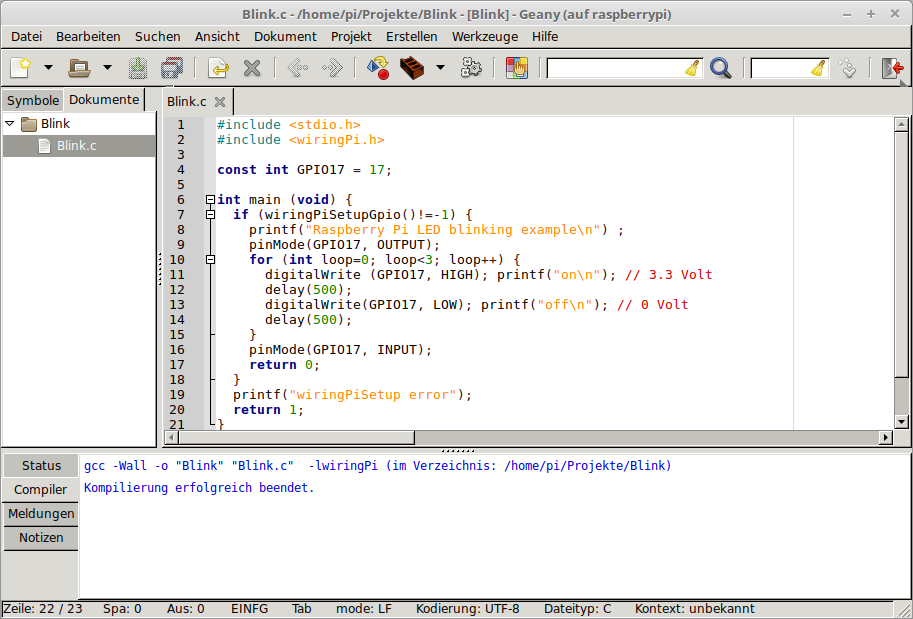
\includegraphics[scale=0.4]{images/Geany_Window.png}
  \caption{Geany Oberfl�che mit Blink-LED Beispiel}
  \label{Geany-window}
\end{figure}

\clearpage
\subsection{wiringPi C-Bibliothek / gpio Kommandozeilenprogramm}
\label{wiringPi}

WiringPi ist eine C-Bibliothek f�r den Zugriff auf Funktionen der GPIOs des Prozessors des Raspberry Pi's. Sie wird unter der GNU LGPLv3 Lizenz angeboten.\\
Die Bibliothek enth�lt auch das Kommandozeilenprogramm "`gpio"'. Es kann genutzt werden, um von der Konsole oder einem Shell-Skript aus auf die GPIOs zugreifen zu k�nnen. Standardm��ig wird eine eigene WiringPi-Nummerierung f�r die Pins verwendet. Wenn man allerdings den Parameter  "`-g"' hinzuf�gt, werden die BCM-Nummern verwendet. Fr�her musste das Programm mit root-Rechten bzw. �ber sudo gestartet werden. Dies ist inzwischen nicht mehr n�tig. Mit dem Befehl "`gpio readall"' kann der aktuelle Status der GPIOs ausgegeben werden. 

\begin{console}
	gpio -v
\end{console} 

\begin{screensmall}
	gpio version: 2.44
	Copyright (c) 2012-2017 Gordon Henderson
	This is free software with ABSOLUTELY NO WARRANTY.
	For details type: gpio -warranty
	
	Raspberry Pi Details:
	Type: Pi Zero, Revision: 03, Memory: 512MB, Maker: Sony 
	* Device tree is enabled.
	*--> Raspberry Pi Zero Rev 1.3
	* This Raspberry Pi supports user-level GPIO access.
\end{screensmall}

\begin{console}
	gpio readall
\end{console} 

\begin{screensmall}
	 +-----+-----+---------+------+---+-Pi Zero--+---+------+---------+-----+-----+
	 | BCM | wPi |   Name  | Mode | V | Physical | V | Mode | Name    | wPi | BCM |
	 +-----+-----+---------+------+---+----++----+---+------+---------+-----+-----+
	 |     |     |    3.3v |      |   |  1 || 2  |   |      | 5v      |     |     |
	 |   2 |   8 |   SDA.1 |   IN | 1 |  3 || 4  |   |      | 5v      |     |     |
	 |   3 |   9 |   SCL.1 |   IN | 1 |  5 || 6  |   |      | 0v      |     |     |
	 |   4 |   7 | GPIO. 7 |   IN | 1 |  7 || 8  | 1 | ALT0 | TxD     | 15  | 14  |
	 |     |     |      0v |      |   |  9 || 10 | 1 | ALT0 | RxD     | 16  | 15  |
	 |  17 |   0 | GPIO. 0 |   IN | 0 | 11 || 12 | 0 | IN   | GPIO. 1 | 1   | 18  |
	 |  27 |   2 | GPIO. 2 |   IN | 0 | 13 || 14 |   |      | 0v      |     |     |
	 |  22 |   3 | GPIO. 3 |   IN | 0 | 15 || 16 | 1 | IN   | GPIO. 4 | 4   | 23  |
	 |     |     |    3.3v |      |   | 17 || 18 | 0 | IN   | GPIO. 5 | 5   | 24  |
	 |  10 |  12 |    MOSI |   IN | 0 | 19 || 20 |   |      | 0v      |     |     |
	 |   9 |  13 |    MISO |   IN | 0 | 21 || 22 | 0 | IN   | GPIO. 6 | 6   | 25  |
	 |  11 |  14 |    SCLK |   IN | 0 | 23 || 24 | 1 | IN   | CE0     | 10  | 8   |
	 |     |     |      0v |      |   | 25 || 26 | 1 | IN   | CE1     | 11  | 7   |
	 |   0 |  30 |   SDA.0 |   IN | 1 | 27 || 28 | 1 | IN   | SCL.0   | 31  | 1   |
	 |   5 |  21 | GPIO.21 |   IN | 1 | 29 || 30 |   |      | 0v      |     |     |
	 |   6 |  22 | GPIO.22 |   IN | 1 | 31 || 32 | 0 | IN   | GPIO.26 | 26  | 12  |
	 |  13 |  23 | GPIO.23 |   IN | 0 | 33 || 34 |   |      | 0v      |     |     |
	 |  19 |  24 | GPIO.24 |   IN | 0 | 35 || 36 | 0 | IN   | GPIO.27 | 27  | 16  |
	 |  26 |  25 | GPIO.25 |   IN | 0 | 37 || 38 | 0 | IN   | GPIO.28 | 28  | 20  |
	 |     |     |      0v |      |   | 39 || 40 | 0 | IN   | GPIO.29 | 29  | 21  |
	 +-----+-----+---------+------+---+----++----+---+------+---------+-----+-----+
	 | BCM | wPi |   Name  | Mode | V | Physical | V | Mode | Name    | wPi | BCM |
	 +-----+-----+---------+------+---+-Pi Zero--+---+------+---------+-----+-----+
\end{screensmall}



\subsection{GPIOZero Python-Bibliothek / pinout Tool}

GPIOZero ist eine der vielen Python Bibliotheken, welche genutzt werden kann
um auf die GPIOs der Raspberry PI zuzugreifen. Sie wird unter der BSD Lizenz 
angeboten.

Das Paket beinhaltet auch das Kommandozeilentool "`pinout"'. Dieses zeigt 
Hardwareinformationen und die Pin-Anordnung in der Kommandozeile an.

\begin{console}
	pinout
\end{console} 

\clearpage
\begin{screensmall}
.-------------------------.
| oooooooooooooooooooo J8 |
| 1ooooooooooooooooooo   |c
---+       +---+ PiZero W|s
 sd|       |SoC|   V1.1  |i
---+|hdmi| +---+  usb pwr |
`---|    |--------| |-| |-'

Revision           : 9000c1
SoC                : BCM2835
RAM                : 512Mb
Storage            : MicroSD
USB ports          : 1 (excluding power)
Ethernet ports     : 0
Wi-fi              : True
Bluetooth          : True
Camera ports (CSI) : 1
Display ports (DSI): 0

J8:
   3V3  (1) (2)  5V    
 GPIO2  (3) (4)  5V    
 GPIO3  (5) (6)  GND   
 GPIO4  (7) (8)  GPIO14
   GND  (9) (10) GPIO15
GPIO17 (11) (12) GPIO18
GPIO27 (13) (14) GND   
GPIO22 (15) (16) GPIO23
   3V3 (17) (18) GPIO24
GPIO10 (19) (20) GND   
 GPIO9 (21) (22) GPIO25
GPIO11 (23) (24) GPIO8 
   GND (25) (26) GPIO7 
 GPIO0 (27) (28) GPIO1 
 GPIO5 (29) (30) GND   
 GPIO6 (31) (32) GPIO12
GPIO13 (33) (34) GND   
GPIO19 (35) (36) GPIO16
GPIO26 (37) (38) GPIO20
   GND (39) (40) GPIO21

For further information, please refer to https://pinout.xyz/
\end{screensmall}

Die Bezeichnung der Pins ist sehr wichtig, da es unterschiedlichste Arten 
gibt die Pins anzusprechen. Die GPIOZero Bibliothek verwendet per Default
die Broadcom Nummerierung (BCM numbering). Das Hei�t will
man den physikalisch dritten Pin (direkt unter den 3.3V) schalten, muss man
wissen dass dieser die Bezeichnung GPIO2 besitzt und demzufolge die Pin-Nummer 2
verwendet werden muss.

Technisch kann das Pin-Schema durch das austauschen der Pin-Factories der GPIOZero 
Bibliothek erreicht werden (\emph{gpiozero.Device.pin\_factory}). Hier wird aber 
nicht n�her auf diese M�glichkeiten eingegangen.


\subsection{wiringPi mit C\# und Mono}

Um mit C\# Zugriff auf Funktionen der GPIOs zu erhalten, wird die wiringPi C-Bibliothek (siehe \ref{wiringPi}) und Mono ben�tigt.\\
Mono ist die quelloffene Implementierung von Microsofts .NET Framework und wird unter der MIT Lizenz angeboten.\\

Damit die C\# Projekte aus Kapitel \ref{Projekte} kompiliert werden k�nnen, ben�tigt man einen Wrapper f�r die wiringPi Funktionen. Nachfolgend ist ein Auszug einer Implementierung eines C\# wiringPi Wrappers angegeben.\\

\lstset{language=C, caption=, label=WiringPiCS, frame=single, basicstyle=\ttfamily
	\footnotesize, breakatwhitespace=false, showstringspaces=false, showtabs=false, tabsize=2 }
\lstinputlisting{source/WiringPi.cs}

Ein vollst�ndiger Wrapper kann z.~B. unter \url{https://github.com/EvilVir/WiringPi.NET/raw/master/Wrapper/WiringPi.cs} bzw. \url{https://goo.gl/isrNeJ} heruntergeladen werden.\\
Am vorbereitet Image ist der Wrapper unter \texttt{/home/pi/Projekte/wiringPi.cs} zu finden.\\


\chapter{Projekte}
\label{Projekte}

\section{LED}

\begin{figure}[ht]
  \centering
  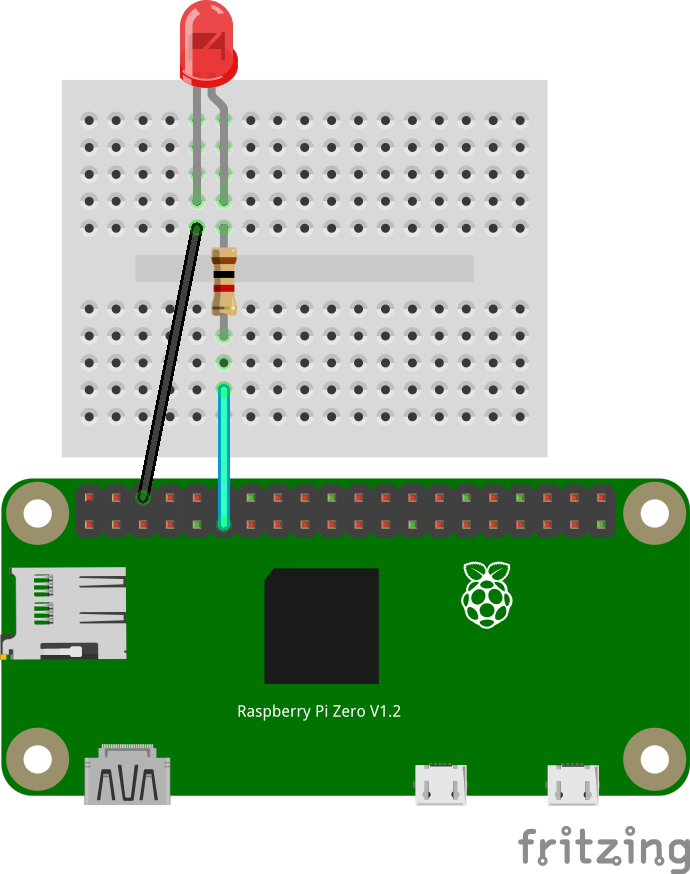
\includegraphics[scale=0.25, angle=-90]{images/LED_Steckplatine.png}	
  %	\caption{}
  \label{LED_Steckplatine}
\end{figure}

\begin{figure}[ht]
	\centering
	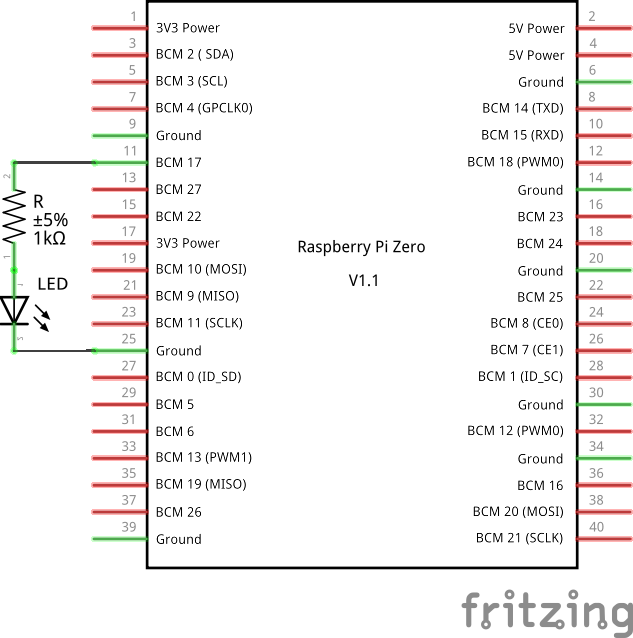
\includegraphics[scale=0.25]{images/LED_Schaltplan.png}	
	%	\caption{}
	\label{LED_Schaltplan}
\end{figure}

\subsection{Shell}

\begin{console}
	gpio -g mode 17 out
	gpio -g write 17 1
	gpio -g write 17 0
	gpio -g mode 17 in
\end{console}

%https://de.scribd.com/doc/101830961/GPIO-Pads-Control2

% gpio drive 0 0  2 mA
% gpio drive 0 3  8 mA <- default
% gpio drive 0 7  16 mA



\subsection{C\#}

\subsection{C}

\begin{console}
	geany &
\end{console}

Nun kann man ein neues Projekt erstellen, dazu w�hlt man \texttt{Projekt} $\rightarrow$ \texttt{Neu...}. Dann Gibt man den Namen des Projekts an, z.~B. PyBlink. Das Anlegen der Verzeichnisse muss man auch noch best�tigen. 

\begin{figure}[ht]
	\centering
	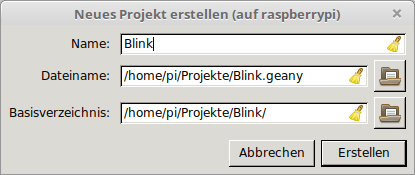
\includegraphics[scale=0.48]{images/Geany_Projekt.png}
	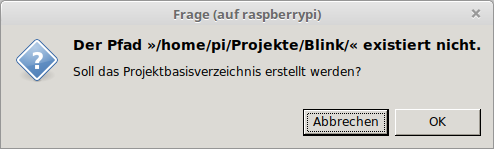
\includegraphics[scale=0.42]{images/Geany_Projekt2.png}
%	\caption{}
	\label{Geany-create}
\end{figure}

Danach w�hlt man \texttt{Datei} $\rightarrow$ \texttt{Speichern unter} um die unbenannte Datei mit dem Namen "`Blink.c"' speichern zu k�nnen. Nun kann man den folgenden C-Source eingeben.

\lstset{language=C, caption=, label=LEDProgram, frame=single, basicstyle=\ttfamily
	\footnotesize, breakatwhitespace=false, showstringspaces=false, showtabs=false, tabsize=2 }
\lstinputlisting{source/Blink.c}

Jetzt darf man nicht vergessen im Men� unter \texttt{Erstellen} $\rightarrow$ \texttt{Kommandos zum Erstellen konfigurieren} die Wiring Pi Library mit "`-lwiringPi"' bei 'Compile' und 'Build' zu erg�nzen.

\begin{figure}[ht]
	\centering
	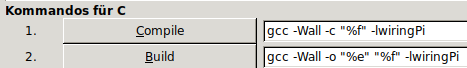
\includegraphics[scale=0.48]{images/Geany_Create_Wiringpi.png}
	%	\caption{}
	\label{Geany-create}
\end{figure}

Nun kann man das Projekt mit den Ziegel-Icon 
\includegraphics[scale=0.4]{images/Geany_Icon_Erstellen.png} erstellen bzw. kompilieren und danach mit dem Zahnrad-Icon 
\includegraphics[scale=0.4]{images/Geany_Icon_Ausfuehren.png} ausf�hren. Beendet wird das Programm mit der Tastenkombination \framebox{Strg}+\framebox{C}. 

\subsection{Python}

\begin{console}
	geany &
\end{console}

Nun kann man ein neues Projekt erstellen, dazu w�hlt man \texttt{Projekt} $\rightarrow$ \texttt{Neu...}. Dann gibt man den Namen des Projekts an, z.~B. PyBlink. Das Anlegen der Verzeichnisse muss man auch noch best�tigen. Danach unter \texttt{Datei} $\rightarrow$ \texttt{Speichern unter} die unbenannte Datei mit dem Namen "`Blink.py"' speichern. Nun kann man den folgenden Python-Source eingeben.

\lstset{language=Python, caption=, 
        label=LEDProgram, frame=single, basicstyle=\ttfamily
	      \footnotesize, breakatwhitespace=false, showstringspaces=false, 
        showtabs=false, tabsize=2 }
\lstinputlisting{source/Blink.py}

Um das Programm auszuf�hren zu k�nnen, muss im Men� unter \texttt{Erstellen}
$\rightarrow$ \texttt{Kommandos zum Erstellen konfigurieren} der Python 
Interpreter von Version 2 auf Version 3 umgestellt werden. Hierf�r einfach im
Textfeld 'Compile' und im Textfeld 'Execute' \texttt{python} durch \texttt{python3}
ersetzen.

\begin{figure}[ht]
	\centering
	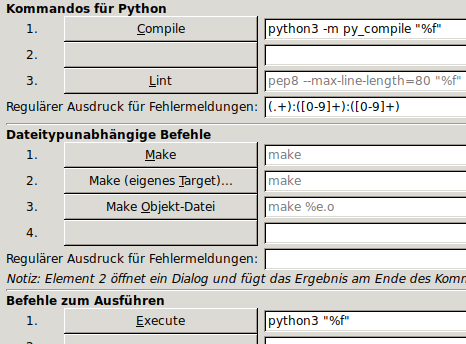
\includegraphics[scale=0.48]{images/Geany_SetPy3.png}
	%	\caption{}
	\label{Geany-setpy3}
\end{figure}

Anschlie�end kann man das Programm mit dem Zahnrad-Icon 
\includegraphics[scale=0.4]{images/Geany_Icon_Ausfuehren.png} ausf�hren. Achtung, nach dem Start braucht die Initialisierung der GPIOZero Library ein paar Sekunden bevor das Programm startet. Beendet wird das Programm mit der Tastenkombination \framebox{Strg}+\framebox{C}.

\subsection{Assembler}
Echte Hardcore-Programmierer k�nnen nat�rlich auch das LED-Beispiel in Assembler 
schreiben\ldots

\lstset{language=[x86masm]Assembler, caption=, 
        label=LEDProgram, frame=single, basicstyle=\ttfamily
	      \footnotesize, breakatwhitespace=false, showstringspaces=false, 
        showtabs=false, tabsize=2 }
\lstinputlisting{source/Blink.asm}


\section{Ampel}

\begin{figure}[ht]
  \centering
  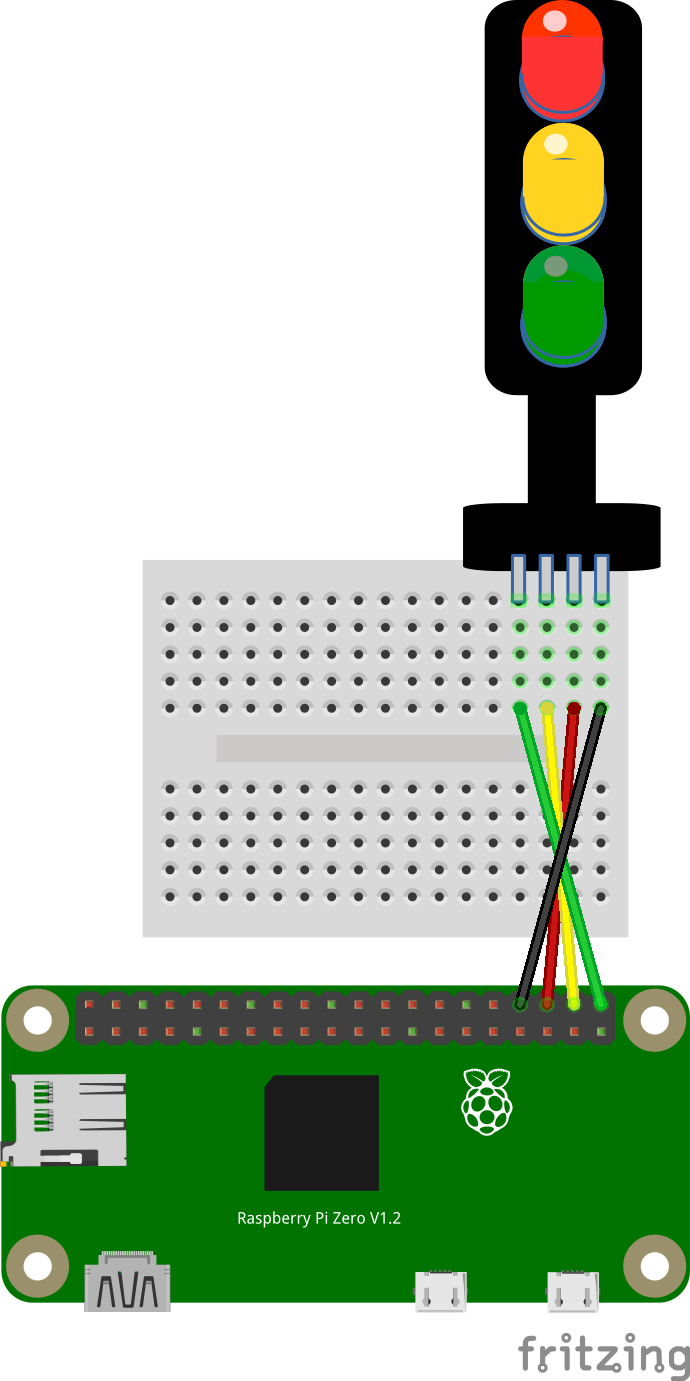
\includegraphics[scale=0.25]{images/TrafficLight_Steckplatine.png}	
  %	\caption{}
  \label{LED_Steckplatine}
\end{figure}

%\begin{figure}[ht]
%	\centering
%	\includegraphics[scale=0.25]{images/TrafficLight_Schaltplan.png}	
%	%	\caption{}
%	\label{LED_Schaltplan}
%\end{figure}

\ExerciseBox{
Bilde die Standardfunktion einer �sterreichischen Ampel nach [Beispiele]\\
Schalte �ber einen Eingang auf Rot f�r den Fu�g�nger�bergang\\
�berwache die CPU-Last und schalte bei �ber 90 \% auf Rot und �ber 50 \% auf Gelb}


\begin{figure}[ht]
	\centering
	
\includegraphics[scale=0.04]{images/Ampel_Rot.png}	
	
\includegraphics[scale=0.04]{images/Ampel_RotGelb.png}
	
\includegraphics[scale=0.04]{images/Ampel_Gruen.png}
	
\includegraphics[scale=0.04]{images/Ampel_Aus.png}
	
\includegraphics[scale=0.04]{images/Ampel_Gruen.png}
	
\includegraphics[scale=0.04]{images/Ampel_Aus.png}
	
\includegraphics[scale=0.04]{images/Ampel_Gruen.png}
	
\includegraphics[scale=0.04]{images/Ampel_Aus.png}
	
\includegraphics[scale=0.04]{images/Ampel_Gruen.png}
	
\includegraphics[scale=0.04]{images/Ampel_Gelb.png}
	%	\caption{}
	\label{Ampel_Ablauf}
\end{figure}


\subsection{C}

\begin{console}
	geany &
\end{console}

Zuerst wird ein neues Projekt erstellt. Dazu w�hlt man im Men�  \texttt{Projekt} $\rightarrow$ \texttt{Neu...}. Dann gibt man den Namen des Projekts an z.~B. TrafficLight. Das Anlegen der Verzeichnisse muss danach auch noch best�tigt werden.
Weitere Einstellungen wie Zeichen f�r Einr�ckungen und Zeilenumbruch k�nnen unter \texttt{Projekt} $\rightarrow$ \texttt{Eigenschaften} vorgenommen werden.\\
Danach w�hlt man \texttt{Datei} $\rightarrow$ \texttt{Speichern unter} um die unbenannte Datei mit dem Namen "`TrafficLight.c"' speichern zu k�nnen. Nun kann man den folgenden C-Source eingeben.

\lstset{language=C, caption=, label=TrafficLightProgram, frame=single, basicstyle=\ttfamily
	\footnotesize, breakatwhitespace=false, showstringspaces=false, showtabs=false, tabsize=2 }
\lstinputlisting{source/TrafficLight.c}

Im Men� unter \texttt{Erstellen} $\rightarrow$ \texttt{Kommandos zum Erstellen konfigurieren} die WiringPi Library mit "`\textit{-lwiringPi}"' bei \texttt{Compile} und \texttt{Build} zu erg�nzen.

\begin{figure}[ht]
	\centering
	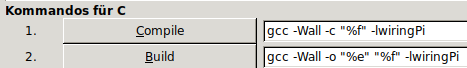
\includegraphics[scale=0.48]{images/Geany_Create_Wiringpi.png}
	%	\caption{}
	\label{Geany-create}
\end{figure}

Nun kann man das Projekt mit den Ziegel-Icon 
\includegraphics[scale=0.4]{images/Geany_Icon_Erstellen.png} erstellen bzw. kompilieren und danach mit dem Zahnrad-Icon 
\includegraphics[scale=0.4]{images/Geany_Icon_Ausfuehren.png} ausf�hren.  

%\clearpage
\subsection{C\#}

\begin{console}
	geany &
\end{console}

Zuerst wird ein neues Projekt erstellt. Dazu w�hlt man im Men� \texttt{Projekt} $\rightarrow$ \texttt{Neu...}. Dann gibt man den Namen des Projekts an, z.~B. csTrafficLight. Das Anlegen der Verzeichnisse muss danach auch noch best�tigt werden. Nachfolgend unter \texttt{Datei} $\rightarrow$ \texttt{Speichern unter} die unbenannte Datei mit dem Namen "`TrafficLight.cs"' speichern. Nun kann man den folgenden C\#-Source eingeben.\\

\lstset{language=C, caption=, label=TrafficLightProgramCS, frame=single, basicstyle=\ttfamily
	\footnotesize, breakatwhitespace=false, showstringspaces=false, showtabs=false, tabsize=2 }
\lstinputlisting{source/TrafficLight.cs}

Um das Programm kompilieren zu k�nnen, muss im Men� unter \texttt{Erstellen}
$\rightarrow$ \texttt{Kommandos zum Erstellen konfigurieren} der Pfad zur Sourcedatei des C\# WiringPi 
Wrapper (siehe \ref{WiringPiCS}) hinzugef�gt werden. Hierf�r im Textfeld \texttt{Kompilieren} den Pfad z.~B. WiringPi.cs erg�nzen.\\
"`\textit{mcs /t:winexe \textquotedblleft\%f\textquotedblright WiringPi.cs /r:System,System.Drawing}"'.\\

\begin{figure}[ht]
	\centering
	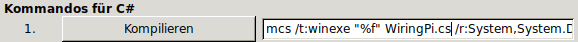
\includegraphics[scale=0.48]{images/Geany_Set_cs.png}
	%	\caption{}
	\label{Geany-setpy3}
\end{figure}

Es muss die WiringPi Wrapper Datei in das Projektverzeichnis kopiert werden. 

\begin{console}
	cp ~/Projekte/WiringPi.cs ~/Projekte/csTrafficLight/
\end{console}

Anschlie�end kann man das Programm mit dem Kompilieren-Icon 
\includegraphics[scale=0.4]{images/Geany_Icon_Kompilieren.png} erstellen bzw. kompilieren und mit dem Zahnrad-Icon 
\includegraphics[scale=0.4]{images/Geany_Icon_Ausfuehren.png} ausf�hren.
Das Programm kann mit der Tastenkombination \framebox{Strg}+\framebox{C} vorzeitig beendet werden.

%\clearpage
\subsection{Python}

Zuerst wird ein neues Projekt erstellt. Dazu w�hlt man \texttt{Projekt} $\rightarrow$ \texttt{Neu...}. Dann gibt man den Namen des Projekts an, z.~B. pyTrafficLight. Das Anlegen der Verzeichnisse muss danach auch noch best�tigt werden. Nachfolgend unter \texttt{Datei} $\rightarrow$ \texttt{Speichern unter} die unbenannte Datei mit dem Namen "`TrafficLight.py"' speichern. Nun kann man den folgenden Python-Source eingeben.\\

\lstset{language=Python, caption=, 
        label=LEDProgram, frame=single, basicstyle=\ttfamily
	      \footnotesize, breakatwhitespace=false, showstringspaces=false, 
        showtabs=false, tabsize=2 }
\lstinputlisting{source/TrafficLight.py}

Anschlie�end kann man das Programm mit dem Zahnrad-Icon

\includegraphics[scale=0.4]{images/Geany_Icon_Ausfuehren.png}  ausf�hren.  

\subsection{Blockly-gPIo}


\begin{figure}[ht]
	\centering
	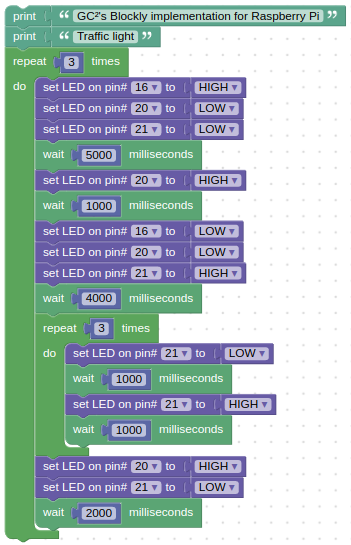
\includegraphics[scale=0.6]{images/Blockly-gPIo_TrafficLight.png}
	%	\caption{}
	\label{Blockly-gPIo_TrafficLight}
\end{figure}




\clearpage
\section{7-Segement Display}


%\textbf{Anschluss:} 

\begin{figure}[ht]
  \centering
  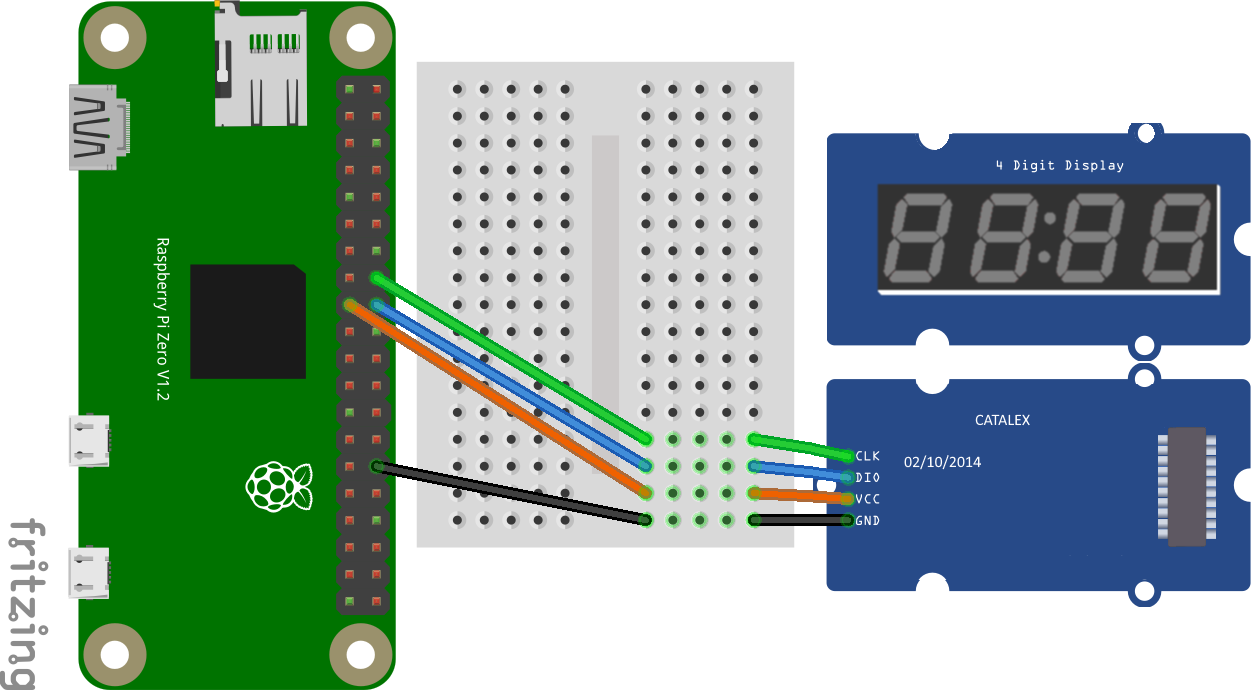
\includegraphics[scale=0.25]{images/TM1637_Steckplatine.png}	
  %	\caption{}
  \label{TM1637}
\end{figure}

\begin{figure}[ht]
	\centering
	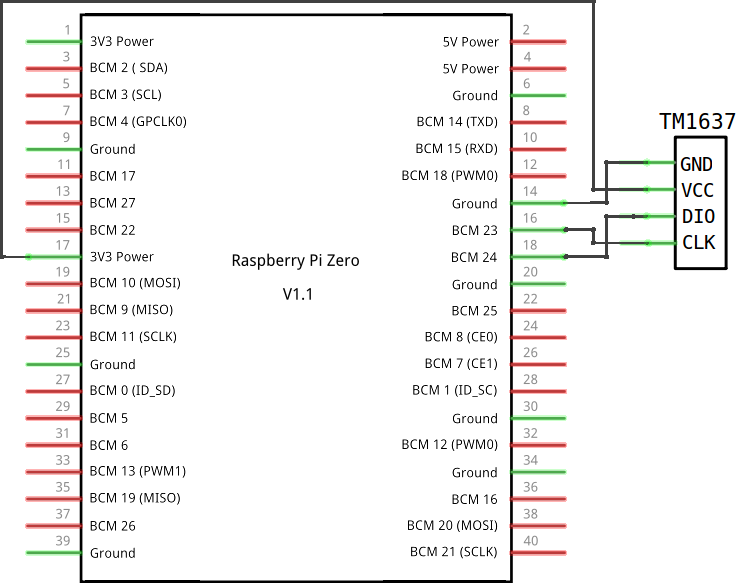
\includegraphics[scale=0.25]{images/TM1637_Schaltplan.png}	
	%	\caption{}
	\label{TM1637}
\end{figure}

\ExerciseBox{
Gib Zahlen und Texte aus [Beispiele]\\
Gib die aktuelle CPU Temperatur aus [Beispiel Python]\\
Gib die gemittelte aktuelle CPU Last in Prozent aus\\
Realisiere eine Laufschrift}

%https://www.mpja.com/download/31227sc.pdf

\textbf{C:} 

\begin{console}
	cd ~/Projekte
	git clone https://github.com/mstroh76/TM1637Display
	cd TM1637Display
	g++ -o TM1637Display *.cpp -lwiringPi
	./TM1637Display
	geany project.geany & 
\end{console}

\textbf{C\#:}

\begin{console}
	cd ~/Projekte
	git clone https://github.com/chirndler/wiringpi.net.sensors.git
	cd wiringpi.net.sensors
	xbuild /p:Configuration=Release wiringpi.net.sensors.sln
	cd bin/Release/
	sudo mono wiringpi.net.sensors.sample.exe 3
\end{console}

\clearpage
\textbf{Python:}
\begin{console}
	sudo pip3 install wiringpi
	git clone https://github.com/depklyon/raspberrypi-python-tm1637.git
	cd raspberrypi-python-tm1637
	sudo python3 setup.py install
\end{console}

\lstset{language=Python, caption=, 
        label=TM1637Program, frame=single, basicstyle=\ttfamily
	      \footnotesize, breakatwhitespace=false, showstringspaces=false, 
        showtabs=false, tabsize=2 }
\lstinputlisting{source/TM1637_Temp.py}

\begin{console}
	python3 TM1637_Temp.py
\end{console}

\subsection{Blockly-gPIo}


\begin{figure}[ht]
	\centering
	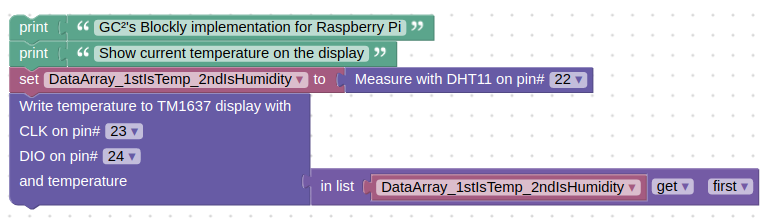
\includegraphics[scale=0.5]{images/Blockly-gPIo_TM1637.png}
	%	\caption{}
	\label{Blockly-gPIo_TM1637}
\end{figure}



\clearpage
\section{Temperatur-/Feuchtesensor DHT22/AM2303}


%\textbf{Anschluss:} 

\begin{figure}[ht]
  \centering
  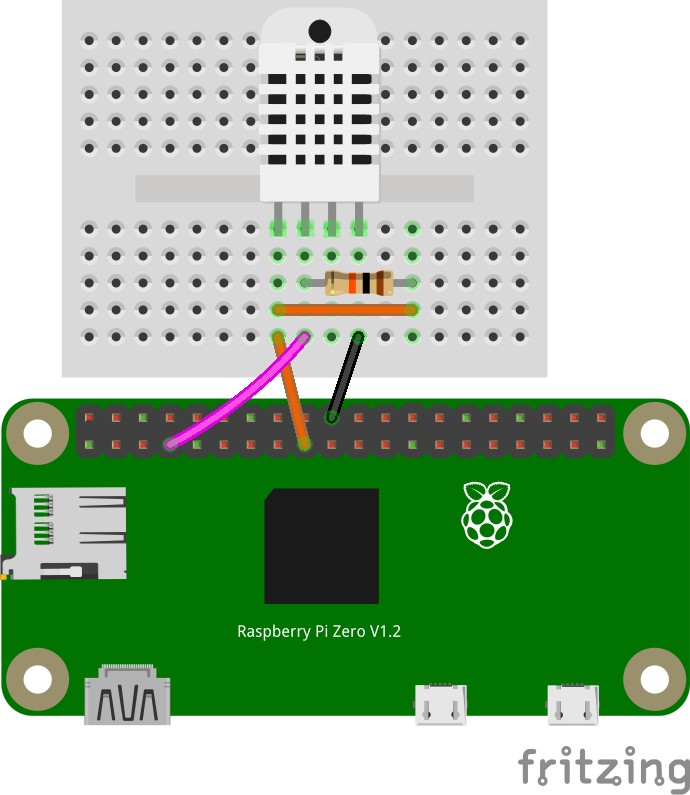
\includegraphics[scale=1.0, angle=-90]{images/DHT22_Steckplatine.png}	
  %	\caption{}
  \label{DHT22_Steckplatine}
\end{figure}

%\textbf{Schaltplan:} 

\begin{figure}[ht]
	\centering
	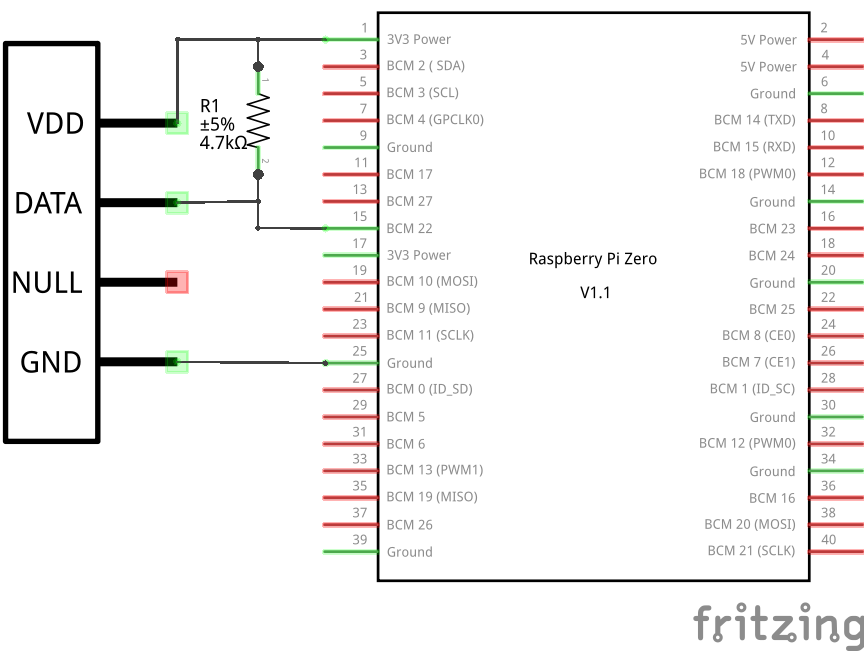
\includegraphics[scale=0.25]{images/DHT22_Schaltplan.png}	
	%	\caption{}
	\label{DHT22_Steckplatine}
\end{figure}


%\textbf{Programm:} 

\begin{console}
cd ~
git clone https://github.com/technion/lol_dht22
cd lol_dht22
./configure
make
sudo ./loldht 7
\end{console}

\clearpage
\section{Distanzsensor HC-SR04}


\begin{figure}[ht]
  \centering
  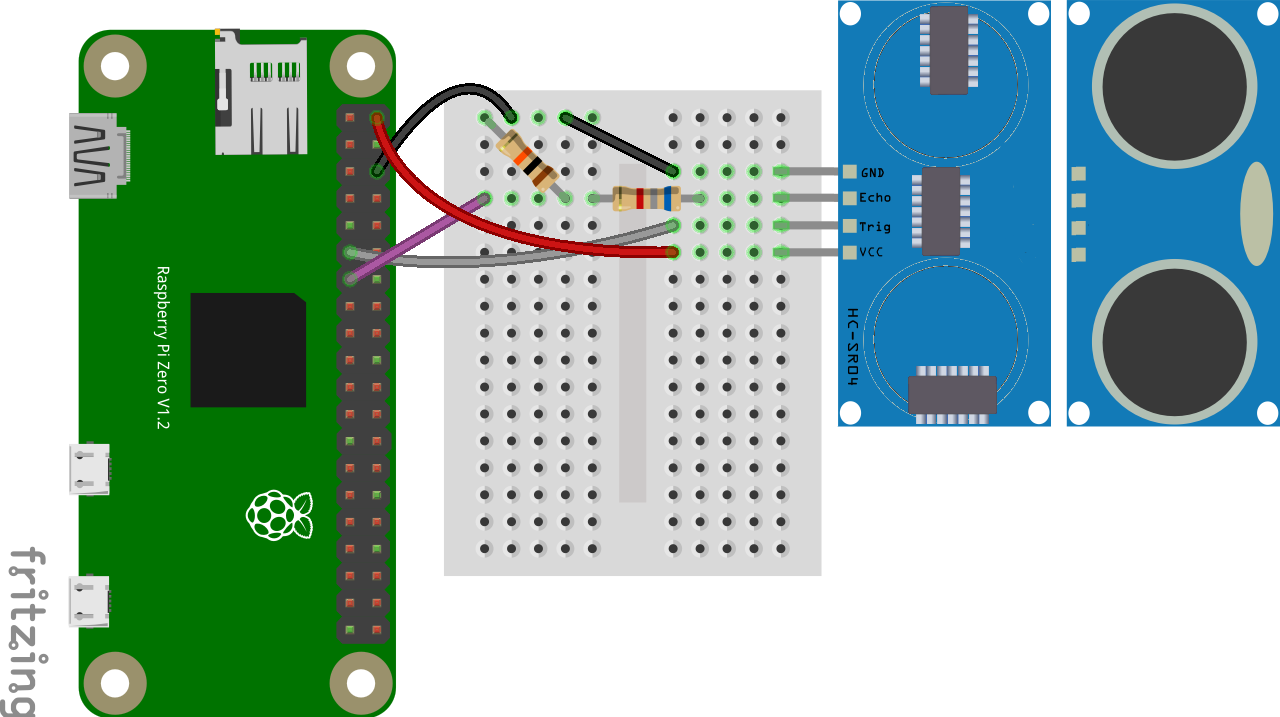
\includegraphics[scale=0.25]{images/HC-SR04_Steckplatine.png}	
  %	\caption{}
  \label{DHT22_Steckplatine}
\end{figure}

\begin{figure}[ht]
	\centering
	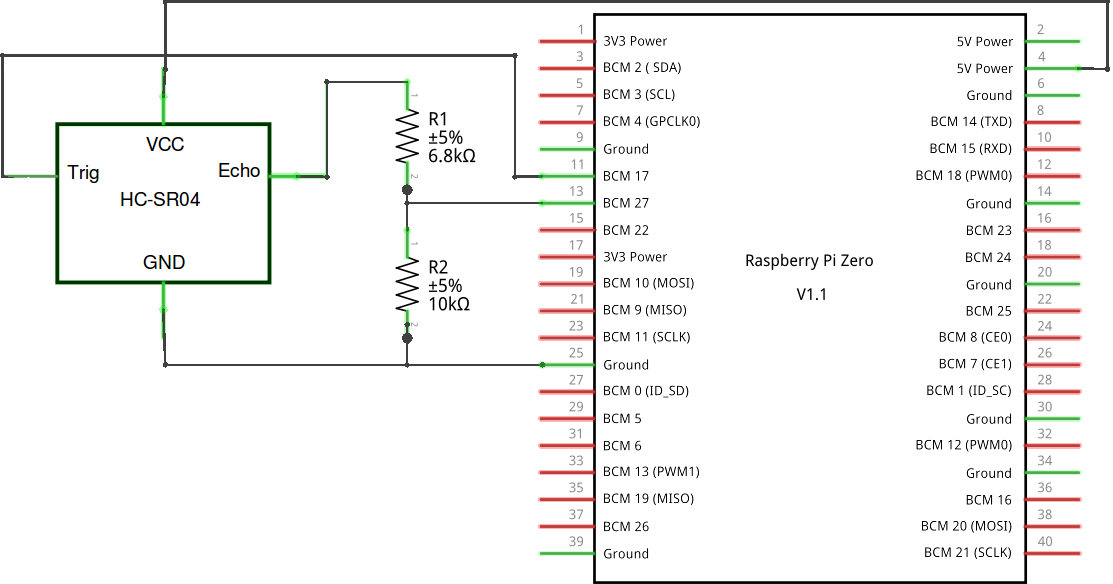
\includegraphics[scale=0.25]{images/HC-SR04_Schaltplan.png}	
	%	\caption{}
	\label{DHT22_Steckplatine}
\end{figure}

\ExerciseBox{
Miss die Distanz [Beispiele]\\
Filtere die gemessene Distanz\\
Ermittle die Geschwindigkeit eines bewegten Objektes\\
Bewerte die Distanz mit der Ampel: Rot niedriger Abstand, Gr�n ausreichender Abstand     
Gib den Wert zyklisch am TM1637 Display aus [Beispiel Python]\\
Verwende die korrigierte Schallgeschwindingkeit bei aktueller Lufttemperatur vom DHT22}


\subsubsection{C}

\begin{console}
	cd ~/Projekte
	git clone https://github.com/mstroh76/Sensors-WiringPi.git
	cd Sensors-WiringPi/HC-SR04	
	g++ -o HC-SR04 *.cpp -lwiringPi	
	./HC-SR04
	cd ..
	geany HC-SR04.geany &
\end{console}


\subsubsection{C\#}

\begin{console}
	cd ~/Projekte
	git clone https://github.com/chirndler/wiringpi.net.sensors.git
	cd wiringpi.net.sensors
	xbuild /p:Configuration=Release wiringpi.net.sensors.sln
	cd bin/Release/
	sudo mono wiringpi.net.sensors.sample.exe 2
\end{console}


\subsubsection{Python}

\lstset{language=Python, caption=, 
        label=HCSR04Program, frame=single, basicstyle=\ttfamily
	      \footnotesize, breakatwhitespace=false, showstringspaces=false, 
        showtabs=false, tabsize=2 }
\lstinputlisting{source/HC_SR04.py}

\begin{console}
	python3 HC_SR04.py
\end{console}


\subsubsection{Blockly-gPIo}

\begin{figure}[ht]
	\centering
	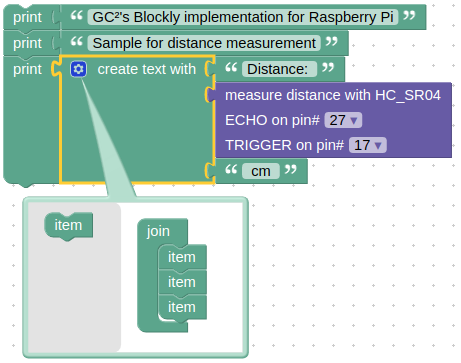
\includegraphics[scale=0.44]{images/Blockly-gPIo_HC_SR04_EN.png}
	\includegraphics[scale=0.44]{images/Blockly-gPIo_HC_SR04_DE.png}
	%	\caption{}
	\label{Blockly-gPIo_HC_SR04}
\end{figure}




\chapter*{Anhang}


\subsection*{GPIO's Raspberry Pi Zero}

\begin{figure}[ht]
  \centering
  \includegraphics[scale=0.55]{images/PiZero.jpg}
  \includegraphics[scale=0.77]{images/PinOut-RPi.png}
  %\caption{}
  %\label{GPIORaspberryPi}
\end{figure}
\clearpage

\section*{Lizenz}
\lhead{}
\chead{}
\rhead{ANHANG}

\begin{figure}[ht]
  \centering
  \includegraphics[scale=1.0]{images/by-sa.png}
\end{figure}

Dieses Werk steht unter der Lizenz Creative Commons BY-SA 3.0 (\url{https://creativecommons.org/licenses/by-sa/3.0/at}). Sie erlaubt ausdr�cklich, das Werk zu vervielf�ltigen, zu verbreiten und �ffentlich zug�nglich machen. Es ist weiters erlaubt diese Werk zu ver�ndern und darauf aufbauen zu erweitern. Es muss allerdings der Urheber genannt werden und die aufbauende Arbeit muss unter der gleichen Lizenz stehen.\\
Die Anleitung enth�lt Teile aus anderen E-Book's des Autors Martin Strohmayer, diese k�nnen �ber\\
Amazon \urlsmall{https://www.amazon.de/-/e/B071HJ6GYJ} und\\
Google \urlsmall{https://play.google.com/store/books/author?id=Martin+Strohmayer}\\
bezogen werden.\\
Wenn sie die Arbeit des Autors unterst�tzen wollen erwerben Sie das E-Book, Danke!\\

Es wurden freie (CC0) Grafiken von Openclipart verwendet \url{https://openclipart.org}.\\ 
Schaltpl�ne und Ansichten Steckplatine wurden mit Fritzing erstellt \url{http://fritzing.org}.
%DHT22, 
Es wurden Fritzing Componenten von Adafruit  \url{https://github.com/adafruit/Fritzing-Library} und 
% HC-SR04
Ricky Ng-Adam %\url{https://github.com/rngadam/ART/tree/master/ele/fritzing} 
und
% Grove
Yihui Xiong \url{https://github.com/mcauser/seeed-fritzing-parts}
 verwendet. Sie werden ebenfalls unter der CC-BY-SA Lizenz zur Verf�gung gestellt. 


\subsection*{Haftungsausschluss}

Die Benutzung dieses Buches und die Umsetzung der darin enthaltenen Informationen erfolgt ausdr�cklich auf eigenes Risiko. Haftungsanspr�che gegen den Verlag und den Autor f�r Sch�den materieller oder ideeller Art, die durch die Nutzung oder Nichtnutzung der Informationen bzw. durch die Nutzung fehlerhafter und/oder unvollst�ndiger Informationen verursacht wurden, sind grunds�tzlich ausgeschlossen. Rechts- und Schadensersatzanspr�che sind daher ausgeschlossen. Das Werk inklusive aller Inhalte wurde unter gr��ter Sorgfalt erarbeitet. Der Verlag und der Autor �bernimmt jedoch keine Gew�hr f�r die Aktualit�t, Korrektheit, Vollst�ndigkeit und Qualit�t der bereitgestellten Informationen. Druckfehler und Falschinformationen k�nnen nicht vollst�ndig ausgeschlossen werden. F�r die Inhalte, der in diesem Buch abgedruckten Internetseiten, sind ausschlie�lich die Betreiber der jeweiligen Internetseiten verantwortlich. Der Verlag und der Autor haben keinen Einfluss auf Gestaltung und Inhalte fremder Internetseiten. Verlag und Autor distanzieren sich daher von allen fremden Inhalten. %Zum Zeitpunkt der Verwendung waren keinerlei illegalen Inhalte auf den Webseiten bekannt.



\end{document}
%EOF
